\chapter{Methodology}
In this chapter we will explore the approaches followed to plan, organise, manage and develop the project. We will discuss the methodologies that were adapted and combined to complete the research and development of the project along with why they were implemented. This section aims to give insight to the reader how the project transformed from research to final software while collaborating as a team.  

% ========================== Development approach  ========================== 
\section{Development approach}
Section on development approach agile v incremental..meetings..story line time line

% ========================== KanBan  ========================== 
\section{KanBan}
The Kanban Method is a means to design, manage, and improve flow systems for knowledge work. The method also allows organizations to start with their existing workflow and drive evolutionary change. They can do this by visualizing their flow of work, limit work in progress (WIP) and stop starting and start finishing.

The Kanban Method gets its name from the use of kanban - visual signaling mechanisms to control work in progress for intangible work products.

% ========================== Version Control  ========================== 
\section{Version Control}
Use of github, branches , KanBan project section to track progress

% ========================== Choice of tech  ========================== 
\section{Choice of tech }
tech used and why
 Selection criteria for algorithms, languages, platforms and technolo-gies.
 
% ========================== Testing , pass fail metrics  ========================== 
\section{Testing , pass fail metrics}
how we planned to test, what did we deternmine wwas a pass or fail

Check out the nice graphs in Figure \ref{tikz:graphs}, and the nice diagram in Figure \ref{tikz:mydiagram}.

\begin{figure}
  \centering
  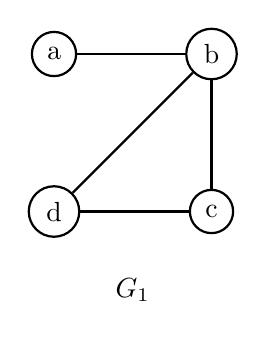
\begin{tikzpicture}
  \begin{scope}[every node/.style={circle,thick,draw}]
  \node (a) at (0,2) {a};
  \node (b) at (2,2) {b};
  \node (c) at (2,0) {c};
  \node (d) at (0,0) {d};
  \end{scope}
  \begin{scope}[every edge/.style={draw=black,thick}]
  \path (a) edge (b);
  \path (b) edge (c);
  \path (b) edge (d);
  \path (c) edge (d);
  \end{scope}
  \node () at (1,-1) {$G_1$};
  \end{tikzpicture}
  \hspace{1.5cm}
  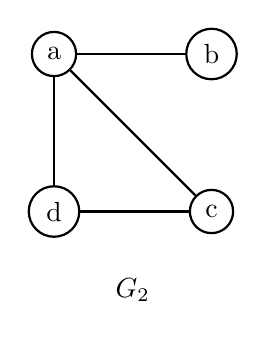
\begin{tikzpicture}
  \begin{scope}[every node/.style={circle,thick,draw}]
  \node (1) at (0,2) {a};
  \node (2) at (2,2) {b};
  \node (3) at (2,0) {c};
  \node (4) at (0,0) {d};
  \end{scope}
  \begin{scope}[every edge/.style={draw=black,thick}]
  \path (1) edge (2);
  \path (1) edge (3);
  \path (1) edge (4);
  \path (3) edge (4);
  \end{scope}
  \node () at (1,-1) {$G_2$};
  \end{tikzpicture}
  \caption{Nice pictures}
  \label{tikz:graphs}
\end{figure}


\begin{figure}
  \centering
  \begin{tikzpicture}[node distance=6cm]
  \node (a) [rect] {A Big Blue Block};
  \node (b) [oval, right of=a] {And His Oval Friend};
  \draw [line] (a) -- (b);
  \end{tikzpicture}
  \caption{Nice pictures}
  \label{tikz:graphs}
\end{figure}